\documentclass{article}
\usepackage{amsmath}
\usepackage{amsthm}
\usepackage{amsfonts}
\usepackage{amssymb}
\usepackage{bbold}
\usepackage{dsfont}
\usepackage{graphicx}
\usepackage{cleveref}
\usepackage{bm}
\usepackage{booktabs}
\usepackage{siunitx}
\usepackage{xcolor}
\usepackage[utf8]{inputenc}
\usepackage[english]{babel}
\newtheorem{definition}{Definition}
\newtheorem{example}{Example}
\newcommand{\exP}[1]{\mathrm{e}^{#1}}
\newcommand{\dif}{\mathrm{d}}
\renewcommand{\vec}[1]{\mathbf{#1}}
\newcommand{\pdagger}{{\phantom{\dagger}}}
\newcommand{\state}[1]{\vert #1\rangle}
\newcommand{\cstate}[1]{\langle #1\vert}
\newcommand{\tr}[1]{\mathrm{tr}\left\{#1\right\}}
\newcommand{\trs}[2]{\, \mathrm{tr}_{#1}\{#2\}}
\newcommand{\expc}[3]{\langle #1\vert #2 \vert #3\rangle}
\usepackage[doi=false,url=false,isbn=false,backend=bibtex,style=nature,natbib=true,sorting=none]{biblatex}
\bibliography{bib.bib}
\usepackage{geometry}
\geometry{
	a4paper,
	total={170mm,257mm},
	left=15mm,
	right=15mm,
	top=15mm,
}
\begin{document}
\title{Report 15: Dynamics in the isolated molecule: Comparison between Ehrenfest and ML-MCTDH}
\author{Rudolf Smorka}
\maketitle
We compare the dynamics in the isolated spinless Peierls model, which is described by the following Hamiltonian
\begin{equation*}
	H_\mathrm{Peierls}/\hbar\omega = \sum_i E_i^\pdagger c_i^\dagger c_i^\pdagger + \sum_\alpha a_\alpha^\dagger a_\alpha^\pdagger -T_0\sum_i (c_i^\dagger c_{i+1}^\pdagger + \mathrm{h.c.}) + T_1\sum_{i}(c_i^\dagger c_{i+1}^\pdagger + \mathrm{h.c.})(a_{i+\frac{1}{2}}^\dagger + a_{i+\frac{1}{2}}^\pdagger)
\end{equation*}
of electrons on a one-dimensional lattice with open boundary condition interacting with bond-vibrations via nearest-neighbor hopping. The parameters are 
\begin{align*}
	\varepsilon_i &= \hbar\omega E_i= -\SI{240}{\milli\electronvolt}\\
	\omega_\alpha &= \SI{2}{\milli\electronvolt}\\
	t_0 &= \hbar\omega T_0= \SI{40}{\milli\electronvolt}\\
	t_1 &= \hbar\omega T_1 = \SI{4}{\milli\electronvolt},
\end{align*}
which are the same as used in the reports on the Fransson model previously. 
The initial state is assumed to be a product state
\begin{equation*}
	\vert \Psi_0\rangle = \vert \psi_0\rangle \vert \phi_0\rangle
\end{equation*}
The electronic system is initialized in the following state
\begin{equation*}
	\vert \psi_0\rangle = \vert 1,0,\dots,0\rangle,
\end{equation*}
corresponding to a single-electron excitation localized on the first site of the lattice. The initial state for the vibrations is a thermal state. To obtain the thermal state, in both Ehrenfest and MCTDH calculations a statistical sampling of the initial wave function is performed. Since in the Ehrenfest method the vibrations are treated as classical particles, their position and momentum is sampled from the thermal Wigner distribution in phase space of the thermal state of the uncoupled one-dimensional harmonic oscillator. In MCTDH, the statistical sampling of the vibrational wave function is performed as developed in \cite{manthe2001partition}. 
\begin{figure}[!h]
	\centering
	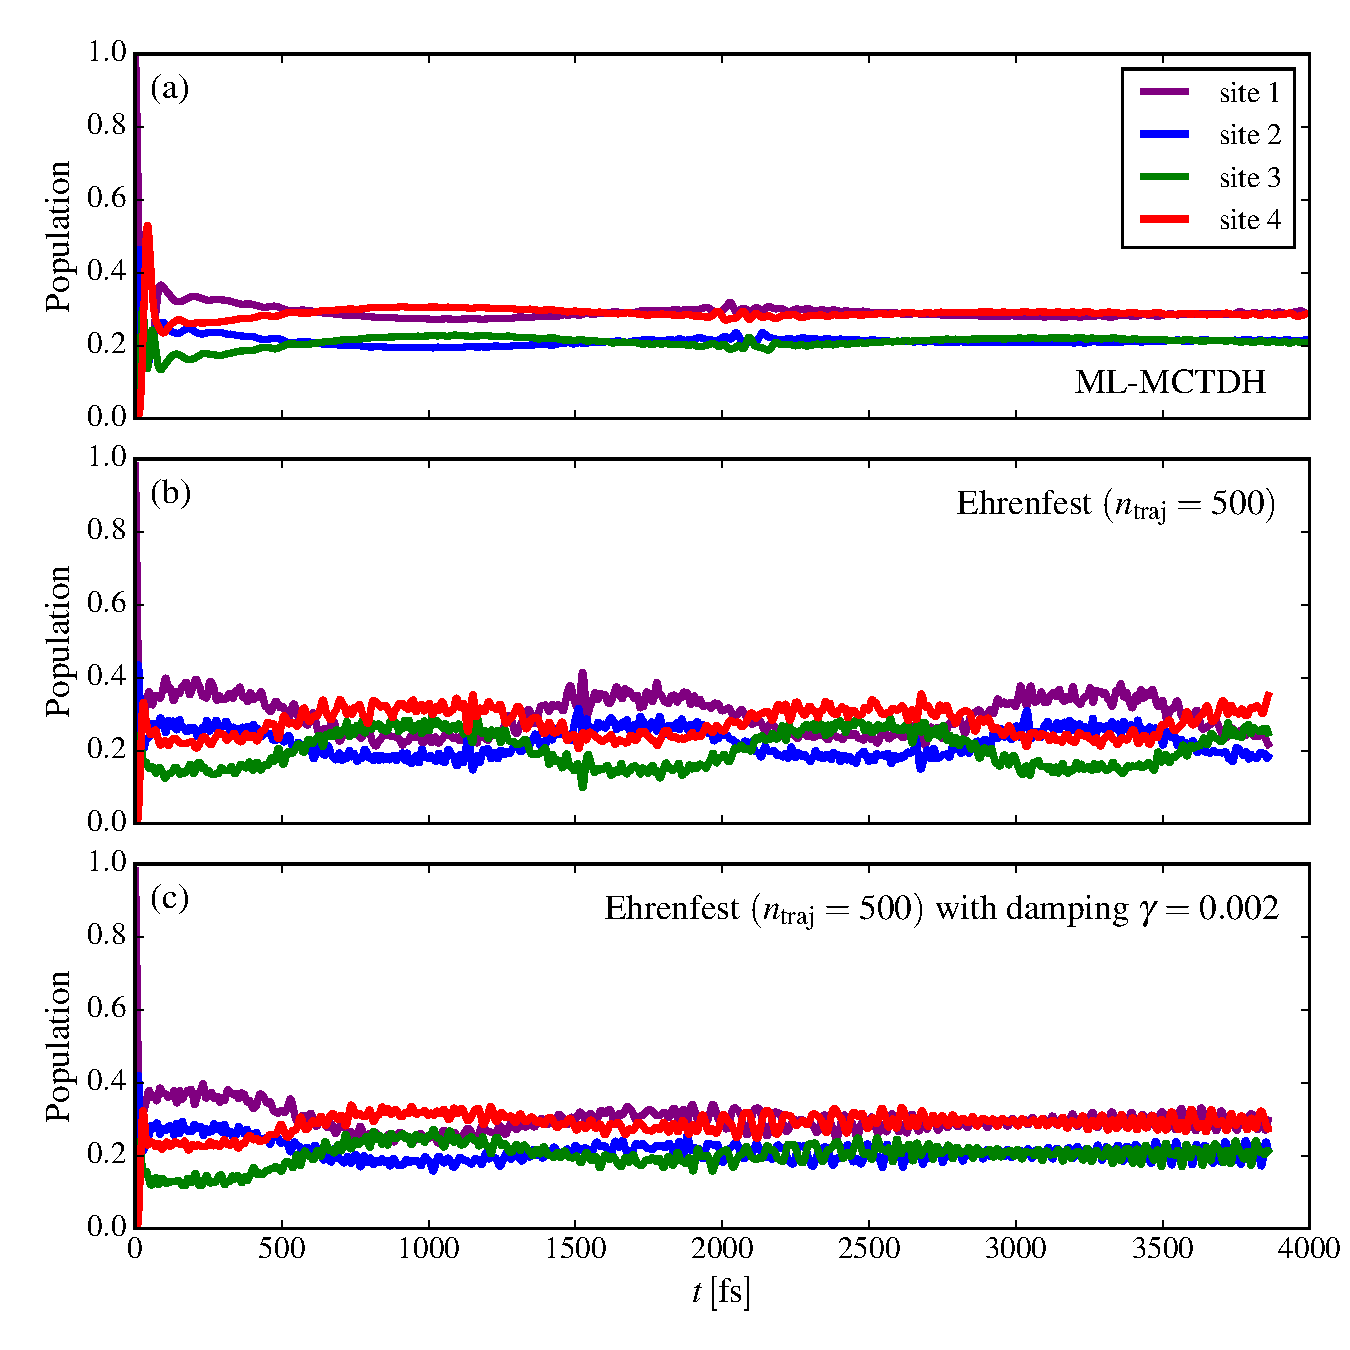
\includegraphics[width=0.8\textwidth]{figs/Peierls_L1x4_MCTDH_v_Ehrenfest.pdf}
\end{figure}
\printbibliography
\end{document}

